\hypertarget{a00010}{
\section{Dokumentacja pliku /home/pawel/Dokumenty/Uczelnia/grupappz/Source/Ass8-server/include/md5/md5.h}
\label{a00010}\index{/home/pawel/Dokumenty/Uczelnia/grupappz/Source/Ass8-server/include/md5/md5.h@{/home/pawel/Dokumenty/Uczelnia/grupappz/Source/Ass8-server/include/md5/md5.h}}
}
{\tt \#include $<$string$>$}\par


Wykres zależności załączania dla md5.h:\nopagebreak
\begin{figure}[H]
\begin{center}
\leavevmode
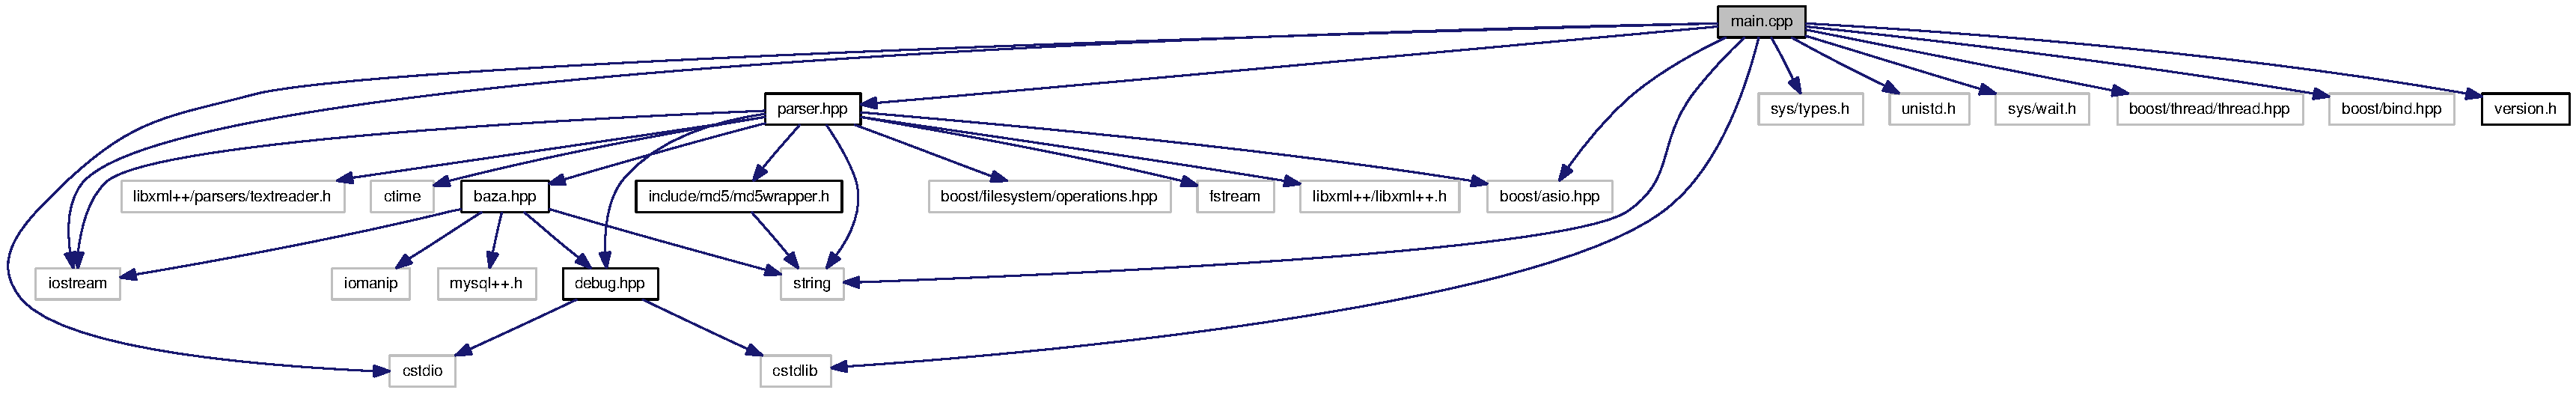
\includegraphics[width=212pt]{a00039}
\end{center}
\end{figure}


Ten wykres pokazuje, które pliki bezpośrednio lub pośrednio załączają ten plik:\nopagebreak
\begin{figure}[H]
\begin{center}
\leavevmode
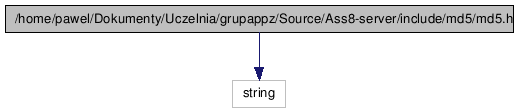
\includegraphics[width=420pt]{a00040}
\end{center}
\end{figure}
\subsection*{Komponenty}
\begin{CompactItemize}
\item 
struct \hyperlink{a00003}{MD5\_\-CTX}
\item 
class \hyperlink{a00002}{MD5}
\end{CompactItemize}
\subsection*{Definicje typów}
\begin{CompactItemize}
\item 
typedef unsigned char $\ast$ \hyperlink{a00010_73204e40637f83518fb695362ea084a4}{POINTER}
\end{CompactItemize}


\subsection{Dokumentacja definicji typów}
\hypertarget{a00010_73204e40637f83518fb695362ea084a4}{
\index{md5.h@{md5.h}!POINTER@{POINTER}}
\index{POINTER@{POINTER}!md5.h@{md5.h}}
\subsubsection[{POINTER}]{\setlength{\rightskip}{0pt plus 5cm}typedef unsigned char$\ast$ {\bf POINTER}}}
\label{a00010_73204e40637f83518fb695362ea084a4}




Definicja w linii 45 pliku md5.h.